%%%%%%%%%%%%%%%%%%%%%%%%%%%%%%%%%%%%%%%%%%%%%%%%%%%%%%%%%%%%%%%%%%
% Sample template for MIT Junior Lab Student Written Summaries
% Available from http://web.mit.edu/8.13/www/Samplepaper/sample-paper.tex
%
% Last Updated August 30, 2011
%
% Adapted from the American Physical Societies REVTeK-4.1 Pages
% at http://publish.aps.org
%
% ADVICE TO STUDENTS: Each time you write a paper, start with this
% template and save under a new filename. If convenient, don't
%    erase unneeded lines, just comment them out.  Often, they
%    will be useful containers for information.
%
% Using pdflatex, images must be either PNG, GIF, JPEG or PDF.
%     Turn eps to pdf using epstopdf.
%%%%%%%%%%%%%%%%%%%%%%%%%%%%%%%%%%%%%%%%%%%%%%%%%%%%%%%%%%%%%%%%%%


%%%%%%%%%%%%%%%%%%%%%%%%%%%%%%%%%%%%%%%%%%%%%%%%%%%%%%%%%%%%%%%%%%
% PREAMBLE
% The preamble of a LaTeX document is the set of commands that precede
% the \begin{document} line.  It contains a \documentclass line
% to load the REVTeK-4.1 macro definitions and various \usepackage
% lines to load other macro packages.
%
% ADVICE TO STUDENTS: This preamble contains a suggested set of
% class options to generate a ``Junior Lab'' look and feel that
% facilitate quick review and feedback from one's peers, TA's
% and section instructors. Don't make substantial changes without
%     first consulting your section instructor.
%%%%%%%%%%%%%%%%%%%%%%%%%%%%%%%%%%%%%%%%%%%%%%%%%%%%%%%%%%%%%%%%%%

\documentclass[aps,twocolumn,secnumarabic,balancelastpage,amsmath,amssymb,nofootinbib]{revtex4}
%\documentclass[aps,twocolumn,secnumarabic,balancelastpage,amsmath,amssymb,nofootinbib]{revtex4-1}
\pdfpagewidth 8.5in
\pdfpageheight 11in

\usepackage{lgrind} % convert program listings to a form includable in a LaTeX document
\usepackage{chapterbib} % allows a bibliography for each chapter(each labguide has it's own)
\usepackage{color} % produces boxes or entire pages with coloredbackgrounds
\usepackage{graphics}      % standard graphics specifications
\usepackage[pdftex]{graphicx} % alternative graphics specifications
\usepackage{longtable}     % helps with long table options
\usepackage{epsf} % old package handles encapsulated post scriptissues
\usepackage{bm}            % special 'bold-math' package
%\usepackage{asymptote} % For typesetting of mathematical illustrations
\usepackage{thumbpdf}
\usepackage[colorlinks=true]{hyperref} % this package should be added after all others
% use as follows: \url{http://web.mit.edu/8.13}
\usepackage{multirow}
\usepackage{subfigure}

% Define a useful new command for writing units
\newcommand{\cd}{$\cdot$}

%
% And now, begin the document...
%

\begin{document}
\title{Optical Pumping of Rb Vapor}
\author{Jay M.\ Lawhorn}
\email{klawhorn@mit.edu}
\date{\today}
\affiliation{MIT Department of Physics}

\begin{abstract}
Optical pumping in rubidium vapor is used to measure the local geo-magnetic field and the Lande $g$ factors for the $^{85}$Rb and $^{87}$Rb isotopes. The ambient magnetic field is measured to have components $B_x=362.5\pm5.1$ mG, $B_y=56.8\pm8.9$ mG, $B_z=199.8\pm1.8$ mG, with an overall magnitude of $417.8\pm4.7$ mG. The Lande $g$ factors are measured to be $g_{f}^{85} = 0.3511\pm0.0009$ and 
$g_{f}^{87} = 0.5233\pm0.0015,$ significantly higher than the literature values. 
\end{abstract}

\maketitle

%\section{Optical Pumping}

Optical pumping was discovered by Alfred Kastler in the early 1950's. It is an essential technique for the creation of masers and lasers. In this experiment it will be used to explore the Zeeman splitting of two rubidium isotopes as well as measure the local geo-magnetic field.

The atomic levels of the $^{87}$Rb are shown in Figure \ref{rb87}. The $5^{2}P_{1/2}$ to $5S$ transition falls in the optical range with a wavelength of 7948 $\mathrm{\AA}$. These transitions are induced by electric dipole transitions through either absorption/stimulated emission or spontaneous emission, which are restricted to transitions that satisfy $\Delta l = \pm 1$, $\Delta f = 0, \pm1$ ($f=0$ to $f=0$ forbidden), and $\Delta m_f = 0,\pm1$. 
\begin{figure}[htb]
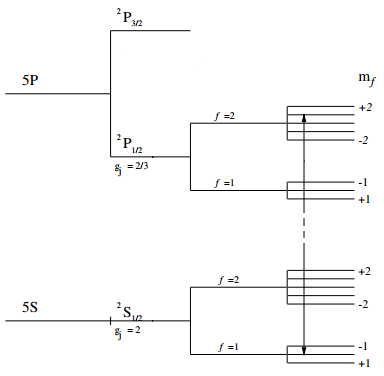
\includegraphics[width=7cm]{rb87.png}
\caption{Energy level diagram for $^{87}$Rb (not to scale). The far right column depicts Zeeman splitting in an ambient magnetic field. The arrow denotes a typical optical transition. Adapted from from \cite{lab}. }
\label{rb87}
\end{figure}

The transitions between the magnetic substates are in the radio frequencies, at approximately 0.5MHz/gauss. They are induced by magnetic dipole transitions, which are restricted by the selection rule $\Delta m_f = 1$. They are induced by thermal collisions and radio frequency photons. 


In thermal equilibrium, the atoms occupy the various magnetic substates according to a Boltzmann distribution law. Optical pumping allows the distribution to be significantly altered. In this case, circularly polarized light from a rubidium lamp is used to pump atoms towards one extreme value of $m_f$. 

This occurs because for electric dipole transitions induced by circularly polarized light with angular momentum $+h$, all allowable transition have $\Delta m_f = +1$. The net result over many cycles of photon absorption and emission is that atoms will disproportionately occupy higher $m_f$ states. Notably, atoms with the highest $m_f$ state allowed will no longer absorb the circularly polarized light because there are no more allowable electric dipole transitions. 

If the atoms are flooded with radio frequency photons at or near the magnetic substate energy difference, the rate of magnetic substate transitions will dramatically increase, allowing for a similar increase in the rate of circularly polarized photon absorption as electric dipole transitions become allowed. 

%\section{Atomic Angular Momentum}

The total atomic angular momentum operators $F^2$ and $F_z$ are defined such that the eigenvalues are
\begin{equation}
\overrightarrow{F}^{2} = f(f+1)\hbar^2, \;\; F_z = m_f \hbar,
\end{equation}
where $f$ is an integer multiple of 1 or $1/2$, and $m_f$ can take on any of the $2f-1$ values from $-f$ to $f$. An atom with total angular momentum $\overrightarrow{F}$ has an atomic magnetic moment $\overrightarrow{\mu}$ given by
\begin{equation}
\overrightarrow{\mu} = \frac{g_f e}{2 m} \overrightarrow{F},
\end{equation}
where $g_f$ is the atomic Lande g-factor, $e$ is the electron charge, and $m$ is the electron mass.

The hyperfine Lande $g$ factor is calculated as
\begin{equation}
g_F \approx g_J \frac{F(F+1)-I(I+1)+J(J+1)}{2F(F+1)}, \label{lande}
\end{equation}
where $g_J=2.00233113(20)$ \cite{amv} is the fine-structure $g$ factor of rubidium, $F=I+J$ is the total atomic angular momentum, $I$ is the nuclear angular momentum, and $J$ is the total electronic angular momentum. For $^{87}$Rb and $^{85}$Rb, $I=5/2$ and $I=3/2$ respectively. From Equation \ref{lande}, the Lande $g$ factors are $g_{f}^{87}=1/2$ and $g_{f}^{85}=1/3$. 

In an external magnetic field, the magnetic substates with different values of $m_f$ split into different energy levels. The energy splitting $\Delta E$ between adjacent magnetic substates is given by 
\begin{equation}
\Delta E = g_f \mu_B B
\end{equation}
where $B$ is the amplitude of the external magnetic field. 

The ratio of magnetic field amplitude to resonant frequency is therefore
\begin{equation}
\frac{B}{f} = \frac{h}{g_f \mu_B},
\end{equation}
and will be the main observable of interest in the later parts of this analysis.

%\section{Apparatus}

The apparatus, shown in Figure \ref{app} consists of a rubidium lamp, a series of optical elements, a vessel containing rubidium gas, and a photodiode. Two sets of Helmholtz coils are centered on the gas vessel and the entire apparatus is covered by a black felt cloth to reduce background light effects. 

\begin{figure}[htb]
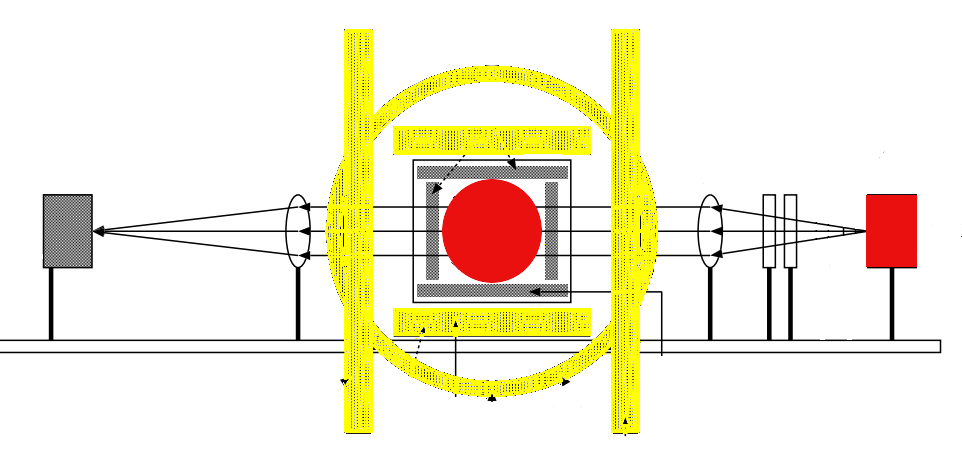
\includegraphics[width=8cm]{rb_setup.png}
\caption{Experimental apparatus. Light from the rubidium lamp (red, left) is circularly polarized and focused into a vessel containing rubidium vapor (red, center). Light that passes through the vapor vessel is then focused into a photodiode (right, grey). The Helmholtz coils (yellow) surround the vapor vessel and provide a uniform magnetic field with in it. Adapted from \cite{lab}. }
\label{app}
\end{figure}

The lamp light is circularly polarized using a linear polarizer and a quarter-wave plate. The two optical components are aligned to produce circularly polarized light by first aligning two linear polarizers at 90$^{o}$ such that no light is transmitted. The two axes of the quarter wave plate are identified by alignment between the two linear polarizers such that there is no transmitted light. The quarter wave plate is then rotated by 45$^{o}$ with respect to its two axes such that light passing through one linear polarizer and the quarter wave plate will be circularly polarized. This is confirmed by rotating the second linear polarizer and observing no change in intensity, indicating circular polarization. The two optical components are mounted on an optical track along with a focusing lens between the rubidium lamp and the rubidium gas vessel. 

The vessel is held at 40$^{o}$ C for all data acquisition by a heating element which is stable to $\pm1^{o}$ C. It contains rubidium vapor as well as neon, a neutral buffer gas which slows the rate of thermal collisions between rubidium atoms and subsequent magnetic substate transitions. The rubidium gas itself is largely comprised of two isotopes: $^{85}$Rb and $^{87}$Rb. 

A second lens is placed on the same optical track on the opposite side of the heated vessel such that the rubidium lamp light passes through the vessel and is then focused onto a photodiode. The current in the photodiode induced by the incident light is converted to a voltage and amplified by a factor of $10^6$. This voltage signal is then passed through a 60 Hz low pass filter and read into an oscilloscope in bandwidth limiting enabled. These two components filter out much of the high frequency noise unrelated to the physical signal. 

An increase in photon absorption in the rubidium gas is detected as a decrease in the photodiode signal, corresponding to a decrease in the number of incident photons. 

The heated vessel is at the center of a set of Helmholtz coils and two sets of radio frequency (RF) coils. The Helmholtz coils are arranged such that there are two coils along three perpendicular axes, with each couple of coils equidistant from the vessel. The z-axis is the optical axis and the x-axis is vertical. Each coil produces a uniform magnetic field in the vessel with magnitude $B$ given by 
\begin{equation}
B = \frac{8\mu_0 N I}{\sqrt{125}R}, \label{b}
\end{equation}
where $N$ is the number of turns in the coil, $I$ is the current, and $R$ is the radius, and $\mu_0=4\pi \times 10^{-7}$ Wb A$^{-1}$m$^{-1}$ is the vacuum permeability. The current through each set of coils is independently controlled by a DC current generator. The coils along the z-axis can optionally be controlled by a programmable function generator instead. 

The RF coils are similarly aligned in sets of two along the three perpendicular axes, and are controlled by a single programmable function generator. 

%\section{Geo-Magnetic Field}

With no applied magnetic field from the Helmholtz coils, the rubidium vapor is sitting in the local geo-magnetic field. The magnitude and direction of the local geo-magnetic field is measured by canceling it with the additional magnetic field from the Helmholtz coils. The resonant RF frequency $f$ of the magnetic substate transitions is given by 
\begin{math}
f = g_f \mu_B B/h
\end{math}
and is linearly proportional to the magnitude of the ambient magnetic field. Thus the magnetic field is minimized by minimizing the resonant frequency. 

The RF coils are set up to sweep out a range of frequencies from $f_{min}$ to $f_{max}$ over a fixed period $T$. The period $T$ was set at 500 ms or 1 s for each sweep in order to minimize the effect of the real-time response of the atoms in the vessel on the time-domain determination of the resonant frequency. The current through the Helmholtz coils aligned with the x-axis, $I_x$, held constant and $I_y$ and $I_z$ fixed at 0. The current $I_x$ has an uncertainty of 2 mA to reflect fluctuations in the generated current. 

The oscilloscope is set to trigger on the function generator's trigger output, which corresponds to when the function generator is producing the lowest frequency in the range. The time corresponding to the minimum of the absorption peak is measured using the oscilloscope cursor, which has a resolution of 2ms. The time delay between the trigger signal and the absorption peak, $\Delta t$ is converted to a frequency using the formula
\begin{equation}
f_{res} = (f_{max}-f_{min})\frac{\Delta t}{T} + f_{min}.
\end{equation}
The uncertainty on the resonant frequency is assessed by linearly propagating the uncertainty on the time measurement of the resonant peak corresponding to the cursor granularity. 

\begin{figure}[htb]
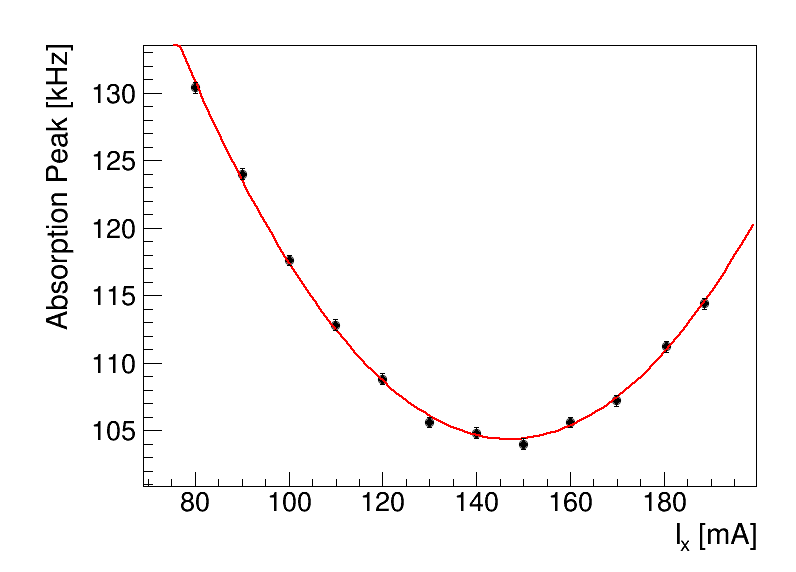
\includegraphics[width=8cm]{x_min1.png}
\caption{Minimum resonant frequency as a function of current through the x-axis Helmholtz coils, $I_x$, with a fit to a quadratic function. }
\label{geo}
\end{figure}

This is repeated for a number of fixed $I_x$ values until a curve such as the one shown in Figure \ref{geo} can be constructed with an observable minimum. Four different curves are constructed for $I_x$: three from the $^{85}$Rb resonance, and one from the $^{87}$Rb resonance. Each curve is fit to a quadratic function, and the current corresponding to the minimum resonant frequency is extracted by calculating $a/2b$ for a quadratic fit of the form $ax^2+bx+c$. The uncertainty in fit parameters is linearly propagated to estimate the overall uncertainty in the minimal current value. The four different measurements are averaged using these uncertainties as weights, and the value for the current that minimizes the resonant frequency is found to be $146.411\pm0.011$ mA.

This current measurement is converted to a magnetic field measurement using Equation \ref{b}, with the uncertainty in the minimal current and physical radius of the Helmholtz coils linearly propagated. The geo-magnetic field in the x-direction is found to be $362.5\pm 5.1$ mG. 

The same process is repeated for the $B_z$ component with $I_x=146$ mA and $I_y=0$ mA. The signal amplitude is markedly reduced due to the smaller net magnetic field. In this region, absorption peaks were also visible at a half and a quarter the frequency of the principle resonant absorption peak. These additional peaks are understood to be artifacts of the function generator, which outputs a signal at a spectrum of frequencies including the target frequency and its higher harmonics. They were observed to be smaller in amplitude than the principle peaks and at exactly half the principle peak frequency, which is consistent with this explanation. The external magnetic field was varied slowly in order to ensure that the primary and secondary peaks were not confused in the event they crossed over each other.
\begin{table}[h]
\caption{\label{min} Frequency sweep parameters and measured current that produces the lowest resonant frequency for each axis and data taking period. The final line for each axis gives the computed average value for the current.}
\begin{tabular}{|c|c|c|c|}
\hline
Axis &Freq Range & Sweep Time &  Current \\
& (kHz)  & (s) & (mA) \\
\hline
$x$ & 80-180& 0.5 & $146.302\pm0.012$  \\
$x$ & 80-130& 1.0 & $147.088\pm0.055$ \\
$x$ & 90-160& 1.0 & $148.501\pm0.083$  \\
$x$ & 90-160& 1.0 & $148.711\pm0.100$  \\
\hline 
$x$ & - & - & $146.411\pm0.011$ \\
\hline
$y$ & - & - & $19.24\pm3$ \\
\hline
$z$ & 0-170 & 1.0 & $35.20\pm 0.42$ \\
$z$ & 0-170 & 1.0 & $35.28\pm 0.08$ \\
$z$ & 0-200 & 1.0 & $34.88\pm 0.74$ \\
$z$ & 0-200 & 1.0 & $34.73\pm 1.02$ \\
\hline
$z$ & - & - & $35.276\pm 0.070$ \\
\hline
\end{tabular}
\end{table}

The effect of the $B_y$ component of the magnetic field was sufficiently small that while a decrease in resonant frequency was observed, no subsequent increase above some minimum was observed. This was tested in two scenarios - first with $I_x=146$ mA and $I_z=35$ mA, and again with $I_x=I_z=0$ mA. Instead, the necessary current was estimated as 19.24 mA, the maximal current the generator could provide, with an uncertainty of 3 mA reflecting the range of currents for which no significant change in resonant frequency was observed. 

A full listing of experimental parameters and calculated current values is given in Table \ref{min}. 

\begin{table}[h]
\caption{\label{bfield} Measured currents and magnetic fields needed to cancel the local geo-magnetic field, as well as physical parameters of the Helmholtz coils. Column 5 gives the nominal experimental values, while column 6 gives the values from the magnetometer. }
\begin{tabular}{|c|c|c|c|c|c|}
\hline
Axis & Current (mA) & N & R (in) & Magnetic  & Mag. \\
& & & & Field (mG) & (mG)\\
\hline
x & $146.411\pm0.011$ & 50 & $14.3\pm0.2$ & $362.5\pm 5.1$ & 380\\
\hline
y & $19.24\pm3$ & 75 & $17.9\pm0.2$ & $56.8\pm8.9$ & 70 \\
\hline
z &  $35.276\pm 0.070$ & 180 & $22.5\pm0.2$ & $199.8\pm1.8$ & 210\\
\hline
\end{tabular}
\end{table}

The magnitude of the geo-magnetic field was measured to be $417.8\pm4.7$ mG. Magnitudes of the individual components are given in Table \ref{bfield}. In order to confirm that the local magnetic field measurement was reasonable, the magnetic field along each coordinate was also measured using a magnetometer with percent level precision. In all cases, the two measurements were consistent to $1.5\sigma$ or less. 


%\section{Resonant Frequencies of Rubidium Isotopes}

To accurately measure the Zeeman splitting parameters of the two rubidium isotopes, the RF signal frequency is fixed and the $B_z$ component of the magnetic field is varied as a sawtooth function of time. The $B_x$ and $B_y$ components were set at the values needed to cancel the geo-magnetic field as measured above. A function generator is used to output a sawtooth function in voltage across the z-axis coils, which is split and read into the oscilloscope. The resistance of the Helmholtz coils along the z-axis is measured to be $49.8\pm0.05$ $\Omega$. From the voltage and resistance, the current through the coils can be calculated. 

A sample dataset is shown in Figure \ref{res}. The two peaks at higher residual magnetic field correspond to the $^{85}$Rb resonance, while the two at lower residual magnetic field correspond to $^{87}$Rb. The oscilloscope readings for the input voltage and the output voltage from the photodiode are saved for three different trigger cycles at each fixed frequency. This is repeated at six different frequencies from 100 kHz to 150 kHz in 10 kHz increments.

\begin{figure}[htb]
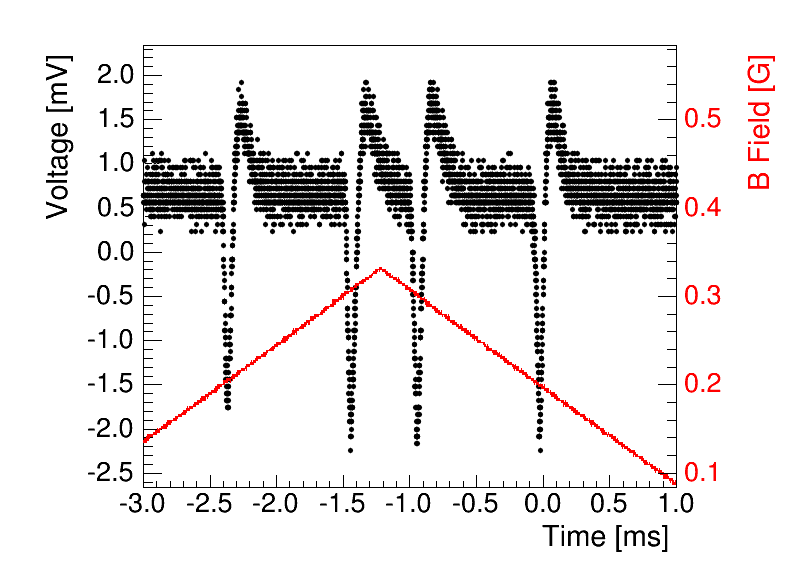
\includegraphics[width=8cm]{abs_peaks.png}
\caption{Sample data taken at fixed frequency and variable magnetic field. The magnetic field amplitude is shown in red after correcting for the measured amplitude needed to cancel the ambient magnetic field. The data is shown in black and shows a significant overshoot after each absorption peak. This is due to the AC coupling of the oscilloscope.}
\label{res}
\end{figure}

For each peak, the magnetic field that optimally allows resonant transitions at the fixed radio frequency is calculated with uncertainty estimated by the peak width. A sample peak is shown in Figure \ref{ext}. Because of the asymmetry of the peak which is expected to be Lorentzian in nature, no fit is performed. Instead, the time of the minimum signal voltage is calculated as the average of the first point in each peak where the voltage takes on the minimum value and the last point where it takes on that same value. The baseline uncertainty in output voltage at each point is equal to half the digitization granularity, while the baseline uncertainty in arrival time is equal to half the time between samples.

The asymmetry of the peaks and overshoot behavior before the return to baseline is due to the AC coupling of the oscilloscope. Any shift in the peak value due to this distortion will be exactly canceled by the shift in the peak on the other side of the maximal applied magnetic field because in one case the peak will be shifted towards higher magnetic field and in the other towards lower by exactly the same amount. Therefore any effect on the overall measurement is negligible because both peaks in a symmetric set are taken into account for each dataset.

\begin{figure}[htb]
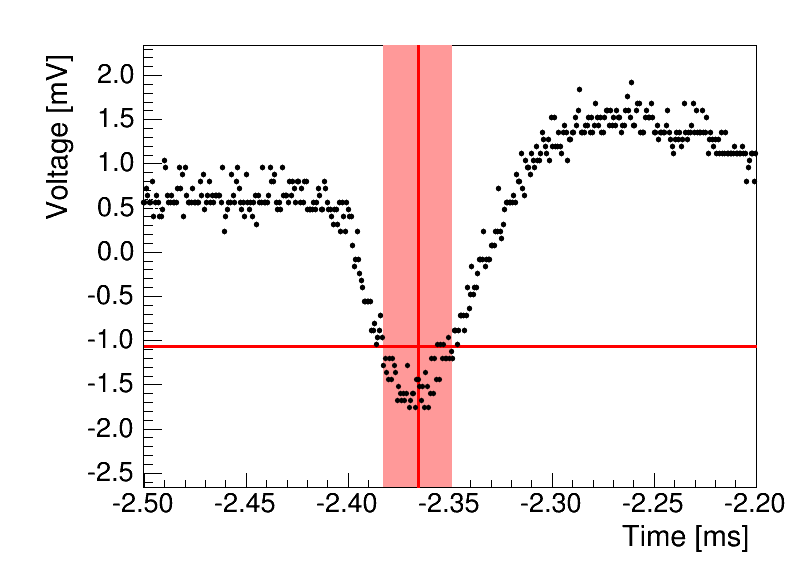
\includegraphics[width=8cm]{peak_area.png}
\caption{Zoomed in view of a single resonant peak. The calculated peak center is denoted by the vertical red line, while the threshold value for the uncertainty on the peak center is denoted by the horizontal red line. The light red region therefore marks the quoted uncertainty on the resonant peak center. }
\label{ext}
\end{figure}

The uncertainty in the peak determination is estimated by finding the first and last points where the values fall below a threshold set at the three times the electronic noise above the minimum signal value. The electronic noise is estimated on a sample by sample basis as the deviation of the first one hundred data points, where no resonant peak structure is observed. The timing of the peak minimum and its uncertainty is converted to a magnetic field strength using the measured input voltage at the corresponding time points. 

Using the known input frequency, the ratio of the resonant frequency $f_{res}$ to the residual magnetic field $|B|$ is computed for each peak, and it should be equal to $h/g_f \mu_B$. The Lande $g$ factor for each isotope is calculated by finding the weighted average of this ratio for peaks corresponding to a single isotope. The measured parameters at each frequency are given in Table \ref{g}. 

The uncertainties in magnetic field strength $B$ and peak location are linearly propagated through to the Lande $g$ factor. The uncertainty in magnetic field strength is generally the limiting uncertainty by a factor of 1.5, though in approximately 10$\%$ of the individual peaks the uncertainty in peak location dominates by an order of magnitude. 

\begin{table}[htb]
\caption{\label{g} Measured values of the ratio of magnetic field strength to frequency and Lande $g$ factors for the six fixed frequencies. }
\begin{tabular}{|c|c|c|c|}
\hline
Freq. & Isotope & $B/f$ & $g_F$ \\
(kHz) & & (G/100kHz) & \\
\hline
100 & $^{85}$Rb & $0.2108\pm0.0012$ & $0.3451\pm0.0020$\\
100 & $^{87}$Rb & $0.1427\pm0.0010$ & $0.5100\pm0.0035$ \\
\hline
110 & $^{85}$Rb & $0.2093\pm0.0013$ & $0.3474\pm0.0021$\\
110 & $^{87}$Rb & $0.1408\pm0.0010$ & $0.5166\pm0.0036$ \\
\hline
120 & $^{85}$Rb & $0.2092\pm0.0020$ & $0.3478\pm0.0033$ \\
120 & $^{87}$Rb & $0.1412\pm0.0025$ & $0.5151\pm0.0090$ \\
\hline
130 & $^{85}$Rb & $0.2081\pm0.0011$ & $0.3496\pm0.0018$ \\
130 & $^{87}$Rb & $0.1400\pm0.0008$ & $0.5195\pm0.0028$ \\
\hline
140 & $^{85}$Rb & $0.2041\pm0.0013$ & $0.3564\pm0.0022$ \\
140 & $^{87}$Rb & $0.1381\pm0.0009$ & $0.5270\pm0.0034$ \\
\hline
150 & $^{85}$Rb & $0.2037\pm0.0010$ & $0.3572\pm0.0018$ \\
150 & $^{87}$Rb & $0.1358\pm0.0008$ & $0.5358\pm0.0030$ \\
\hline
\end{tabular}
\end{table}

Combining the measurements listed in Table \ref{g}, the Lande $g$ factors are found to be
\begin{equation}
\begin{split}
g_{f}^{85} = 0.3511\pm0.0009 \\
g_{f}^{87} = 0.5233\pm0.0015.
\end{split}
\end{equation}
Both of these values are larger than the theoretical predictions from Equation \ref{lande} and literature value \cite{amv} by many times the uncertainty in the measurement. They are however consistent to approximately $2\sigma$ with previous measurements using the same apparatus last year \cite{pras}. 

One explanation for this is that the geo-magnetic field was improperly canceled, resulting in a larger magnetic field than expected at each data point. An additional 80 mG field in the x- or y- directions would lower the $g_f$ values enough to be consistent with literature values, which is approximately equal to the measured magnitude along the y-axis. This was calculated by taking the accepted values for $g_F$ and finding the predicted magnetic field needed to produce a resonance at a given frequency then confirming that adding this additional magnetic field at the beginning of the data analysis chain gave a consistent $g_f$ value. Considering this residual magnetic field could be distributed across all three axes, this seems like a plausible source of the discrepancy. Further measurements with finer resolution of peak motion, especially for the y-component could confirm or rule out this source of discrepancy. 

It could also be that there is some characteristic response time to a change in the frequency of the RF photons during the geo-magnetic field determination portion of the experiment that led to a misidentification of the true resonant frequency in each condition. However, this would have to be about 300 ms to completely explain the discrepancy, which is inconsistent with the observed recovery time for individual peaks on the order of 1 ms. 

While the residual magnetic field is the most plausible single source of the observed inconsistency, other systematic effects such as time-dependent variations in the ambient magnetic field could also contribute as well.

\begin{thebibliography}{3}

\bibitem{lab}
8.14 staff, \emph{Optical Pumping} Lab Guide, February 2011. 

\bibitem{amv}
Arimondo, E., Inguscio, M., Violino, V. \emph{Experimental determination of the hyperfine structure in the alkali atoms}, Rev. Mod. Phys. V \textbf{49 }, Jan. 1977, 31-75. 

\bibitem{pras}
Venkataram, P.S. \emph{Optical Pumping of Rubidium Vapor Atoms}, accessed from \url{http://web.mit.edu/pshanth/www/oppump_psv.pdf}. 

\end{thebibliography}

\end{document}
